%!Tex Root = ../main.tex
% ./Packete.tex
% ./Design.tex
% ./Deklarationen.tex
% ./Aufgabe1.tex
% ./Aufgabe2.tex
% ./Aufgabe3.tex
% ./Aufgabe4.tex
% ./Bonus.tex

\section{General Information}

\begin{frame}{General Information}{Lecture}
  \begin{itemize}
    \item {\large \uppercase{\alert{no need}}} to submit exercise sheets, you get the \alert{Studienleistung} by \alert{passing the exam}
    \item \alert{exam} at 9th of september 2023 (09/09/2023)
  \end{itemize}
  \begin{figure}
    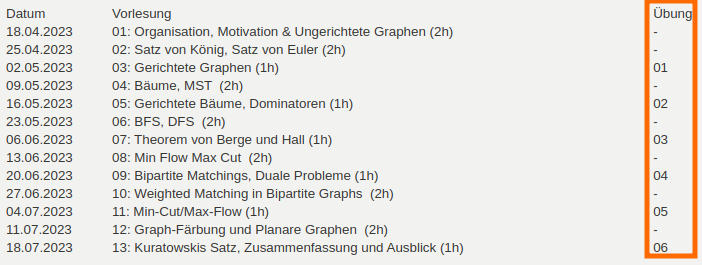
\includegraphics[width=0.6\textwidth]{./figures/dates.png}
    \caption{Dates when exercise classes take place}
  \end{figure}
\end{frame}

\begin{frame}{General Information}{Exercise class}
  \begin{itemize}
    \item The exercise classes get \alert{recorded}: \url{https://youtube.com/playlist?list=PLmsC317bB1b0m9-ZCKGNR6iM6UTPUO__r}
    \item \alert{Feedback} for the exercise class: \url{https://forms.gle/JCcp3qohaAQVswHL6}
    \item \alert{Mindmap} about the topics of the lecture: \url{https://github.com/matthejue/Mindmaps/releases/download/main/Graph_Theory.pdf}
  \end{itemize}
\end{frame}
